\chapter{全景漫游与人的关系}

\section{全景漫游的生理行为特性}
实现全景漫游与传统人机界面最大的区别在于全景漫游时的设备(包括 VR 眼镜或专用眼罩)距离人眼只有 2~3 公分距离,设备整体对人眼呈包裹状态。使用者仅可通过听觉和其他一些不够灵敏的感觉来感受外界环境,使用环境的舒适性就变得非常重要。

全景漫游与人体关联的感觉和生理运动大致有:视觉、听觉、肢体运动等。如图\ref{fig:human_sence}。

\begin{figure}[htp]
\centering
\fbox{
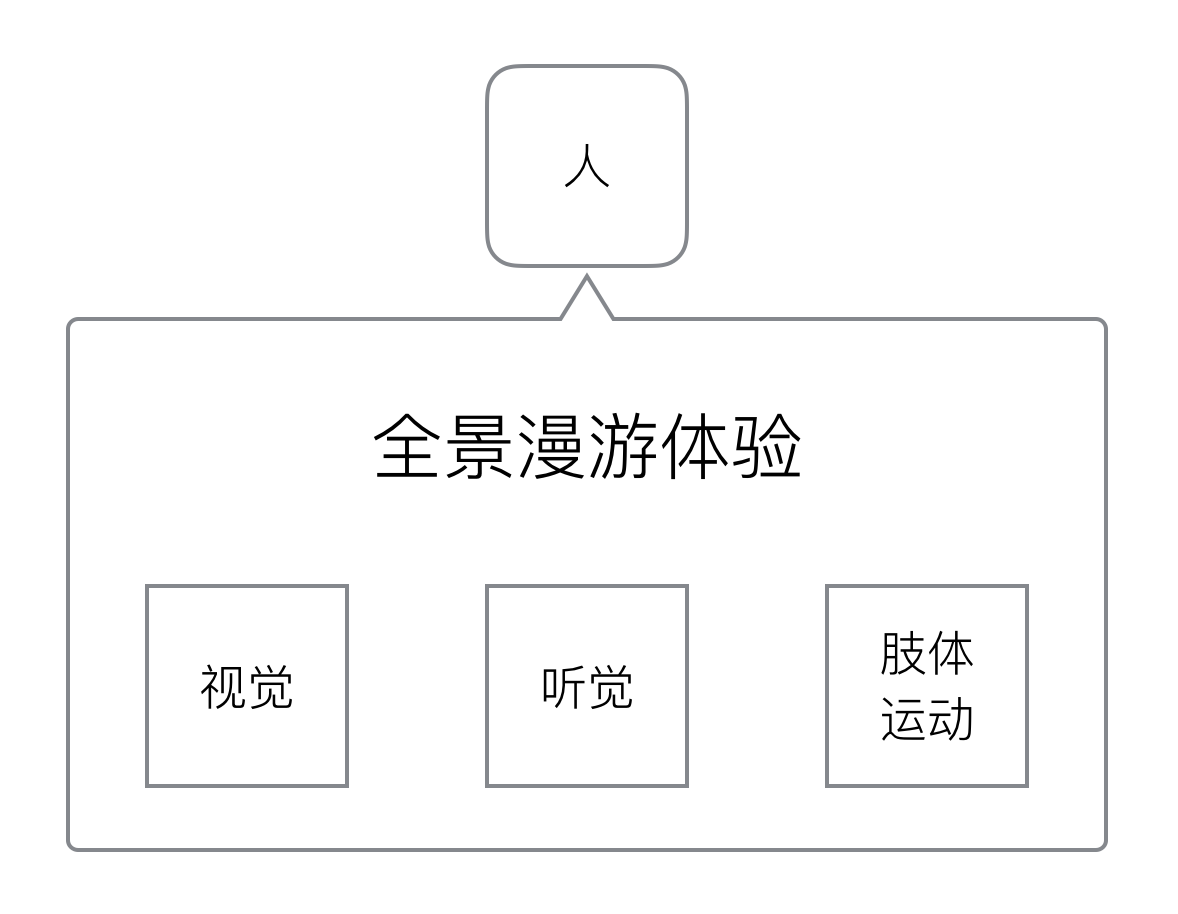
\includegraphics[width=.5\textwidth]{human_sence}
}
\caption{全景漫游与人体知觉}
\label{fig:human_sence}
\end{figure}

\subsection{全景漫游的视觉特征}
全景漫游对人体最大的刺激来源即是视觉刺激,其特征为距离眼睛距离近,色彩、明暗、动作变化等刺激较一般显示屏幕会更为剧烈。

\subsubsection{视角与视野}

人的视角是确定被看物尺寸范围的两端点光线射入眼球的相交角度。视角的大小与观察距离及被看物体上两端点的直线距离有关,其计算公式\ref{eq:angle}如下:
\begin{equation}
\alpha=2\arctan{\frac{D}{2L}}
\label{eq:angle}
\end{equation}

其中,$\alpha$ 为视角,用 $(^{\prime})$ 表示,即$(1/60)^{\circ}$单位;D 为被看物体上两端点的直线距离;L 为眼睛到被看物体的距离。
如果设眼球距镜片距离为 1.5cm,而镜片上一物体显示高度为 2cm,则带入公式可得\ref{eq:data}

\begin{equation}
\alpha=2\arctan{\frac{2cm}{2*1.5cm}}\approx 67.38 ^{\circ} = 2 \times 38.69^{\circ}
\label{eq:data}
\end{equation}

即上下视角各约为 $38.69^{\circ}$,查阅数据可知人在垂直平面的视野最大视区为视平线以上 $50^{\circ}$ 和视平线以下 $70^{\circ}$,颜色辨别界限为视平线以上 $30^{\circ}$,视平线以下 $40^{\circ}$。

由上述计算可知,在使用全景漫游设备观看场景时,假设高为 2cm 的显示物体在人视野中上部已超出颜色辨别界限,下部也已接近颜色辨别界限。物体上部比下部更接近垂直平面内的视野极限,如图\ref{fig:angle}。由此可知,全景漫游场景设计中应将主要元素置于屏幕中央,次要元素尽可能置于屏幕下方以便识别操作。同时,色彩丰富且饱和度高的元素也应置于视野中部,而一些操作类的元素则不应用过于丰富饱和的色彩缀饰,以免让使用者应难以分辨色彩而操作出错。

\begin{figure}[htp]
\centering
\fbox{
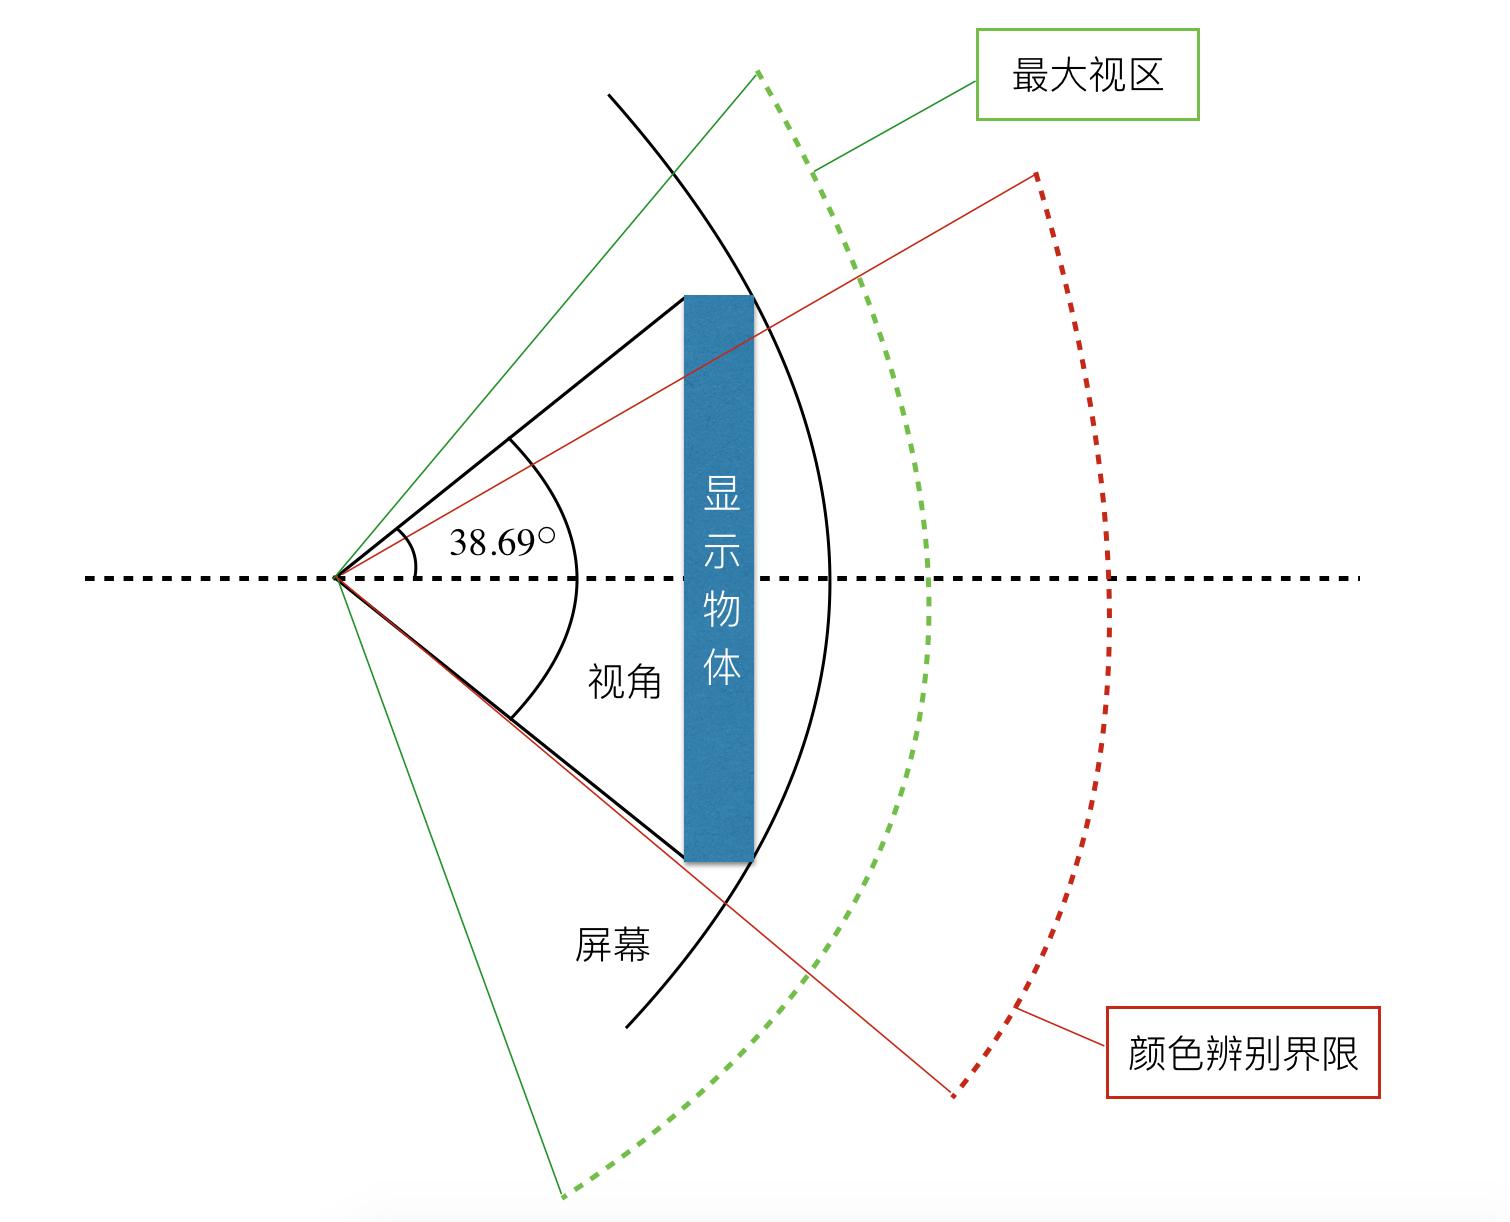
\includegraphics[width=.7\textwidth]{angle}
}
\caption{全景漫游中视野的角度关系}
\label{fig:angle}
\end{figure}

\subsubsection{视觉适应}

配戴全景漫游设备进行观察时,屏幕距眼球距离不足 2cm,属于视距过近状态,应当避免长时间操作,否则易引起眼睛疲劳。同时由于屏幕与眼球距离过近,屏幕亮暗对眼球刺激比通常工作环境更为强烈。当屏幕上场景切换间明暗变化过快时,人眼需要一定的适应时间才能正常分辨,但由于全景漫游设备等封闭性,无法较轻易地脱离这种明暗急剧变化的环境,则眼睛无法得到充足有效的适应时间,则很容易产生视觉疲劳,影响视觉能力。

\subsection{全景漫游的听觉特征}

全景漫游的视觉是主要人体感觉,但听觉是仅此于视觉的重要感觉,尤其是在视觉被全景场景完全包裹住的情况下。

现有全景漫游设备有的自带耳机设备,也有的需要自行配备耳机。但长远来看,配备耳机可能是必然的选择。因为人耳具有“方向敏感度”(或称“双耳效应”),即:声波在进入鼓膜时,受人体的反射、折射和衍射而扭曲变形,大脑能根据经验判断出声源的方位和距离。而前文所说的“耳听八方”即说的是这种能够重建场景音效的能力。

为了“制造”出能够“蒙骗”大脑使其误以为使用者身处虚拟场景中的体验,大致方向是重建出空间任意一点至双耳处的滤波器函数。我们不必去关心空间中某一点的声波是如何传播到人耳中的,只需要将该点声波信号经过滤波器便可以得到它在人耳处的声波信号,如图\ref{fig:hrtf}。而这个信号是可逆的,即被人耳捕捉到之后便由大脑还原成相应位置的“声信号”,从而达到“欺骗”大脑的目的。这个领域的研究对象叫做 HRTF(Head Related Transfer Function):头相关变换函数,是一种音效定位算法。但每个人的听觉能力都是不同的,所以 HRTF 对人类整体并没有通解,而只有对于人类个体经过反复实验测试后的特解。

\begin{figure}[htp]
\centering
\fbox{
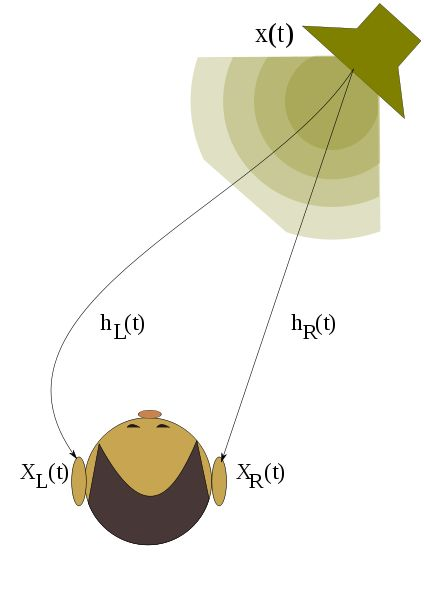
\includegraphics[width=.4\textwidth]{hrtf}
}
\caption{头相关变换函数 HRTF}
\label{fig:hrtf}
\end{figure}

国内外已有厂商根据相关理论设计并制作出了 VR 耳机,可配合 VR 眼镜使用,也可独立使用,它会追踪使用者的姿态、位置变化等,进而计算并还原出模拟三维场景内的声音分布,让使用者仿佛置于真实的场景之中。